\documentclass{beamer}
\usepackage{ulem}
\usepackage{tikz}
\usepackage{booktabs}
\usepackage{graphicx,threeparttable,caption}
\usetikzlibrary{shapes,snakes}
\usepackage[beamer,customcolors]{hf-tikz}
\usepackage{nicematrix}
\usepackage{xcolor}
\usepackage{makecell}
\usepackage{array}
\usepackage{csquotes}
\usepackage{csquotes}
\usepackage{minted}
\usepackage{animate}
\captionsetup{labelformat=empty,labelsep=none}

\graphicspath{ {./png/} }

\usetikzlibrary{
    arrows,
    arrows.meta,
    shapes,
    positioning,
    shadows,
    trees,
    calc
}

\tikzset{%
    >={Latex[width=2mm,length=2mm]},
    % Specifications for style of nodes:
    plain/.style = {},
    base/.style = {
        plain,
        rectangle, rounded corners, draw=black,
        minimum width=1cm, minimum height=1cm,
        text centered, font=\sffamily\tiny\bfseries,
        fill=white, align=center
    },
    app/.style = {base, ellipse},
    data/.style = {base, fill=gray!30},
    action/.style = {base, circle, fill=red!30},
    note/.style = {app, fill=yellow},
    hl/.style={
    set fill color=red!80!black!40,
    set border color=red!80!black
    }
}


\AtBeginSection[]{
  \begin{frame}
  \vfill
  \centering
  \begin{beamercolorbox}[sep=8pt,center,shadow=true,rounded=true]{title}
    \usebeamerfont{title}\insertsectionhead\par%
  \end{beamercolorbox}
  \vfill
  \end{frame}
}
\setbeamercolor{alerted text}{fg=red}
%\usecolortheme[orchid]{structure}
\usetheme[hideothersubsections]{PaloAlto}
\makeatletter
\patchcmd{\csq@bquote@i}{{#6}}{{\emph{#6}}}{}{}
\makeatother
%\usecolortheme{orchid}
%\usefonttheme{professionalfonts}
\newcommand{\soutthick}[1]{%
   \textcolor{red}{
   \renewcommand{\ULthickness}{1pt}%
      \sout{#1}%
   \renewcommand{\ULthickness}{.4pt}% Resetting to ulem default
   }
}
\newcommand{\centered}[1]{\begin{tabular}{l} #1 \end{tabular}}
\setbeamertemplate{section in toc}[square]
\setbeamertemplate{subsection in toc}[square]
\setbeamertemplate{section in sidebar}[shaded]
\setbeamertemplate{items}[square]
\setbeamercovered{transparent} 

\title[]{Introduction to Computational Social Science}
\subtitle{Working with the GDELT API}
\author[]{Mikołaj Biesaga\\ \small{\color{blue}{\href{mailto:m.biesaga@uw.edu.pl}{m.biesaga@uw.edu.pl}}}}
\institute{
\includegraphics[width = 4 cm]{uw.png}}
\date{April 29, 2025}
\begin{document}
\begin{frame}
   \titlepage
\end{frame}

\section[GDELT Project]{What is GDELT Project?}

\begin{frame}
   \frametitle{What is the GDELT Project?}
   \only<1>{
      \begin{definition}
         Global Database of Events, Language, and Tone (GDELT) project is a
         repository of global events and news articles. The GDELT Project monitors
         a \alert{sample} of the world's broadcast, print, and web news from nearly every
         corner of every country in over 100 languages and identifies the people,
         locations, organizations, themes, sources, emotions, counts, quotes,
         images and events driving our global society every second of every day,
         creating a free open platform for computing on the entire world.
      \end{definition}
   }
   \only<2>{
      \begin{itemize}
         \item It is updated every \alert{15 minutes}.
         \item Realtime translation of \alert{65 languages}.
         \item Three main data streams:
         \begin{enumerate}
            \item Physical activities (events) codified in 300 categories;
            \item Entities (people, organizations, places) and emotions;
            \item Visual narratives of the world's news imaginery.
         \end{enumerate}
         \item Sources, from hundreds of thousands of global media outlets to special collections like 215 years of digitized books, 21 billion words of academic literature spanning 70 years, human rights archives and even stream of almost 100 television stations across the US.
      \end{itemize}
   }
   \only<3>{
      \framesubtitle{CAMEO}
      \begin{itemize}
         \item CAMEO (Conflict and Mediation Event Observations) is a coding scheme for events.
         \item There is a list of 20 main categories of events, such as:
         \begin{enumerate}
            \item Make Public Statements;
            \item Appeal;
            \item Express Intent to Cooperate;
            \item ...
         \end{enumerate}
         \item Each event is coded with a CAMEO code, which consists of 3-4
         digits.
         \item For example, the CAMEO code 01 coresponds to Make Public Statements and 018 Make Emphatethic Comment.
      \end{itemize}
   }
   \only<4>{
      \framesubtitle{CAMEO}
      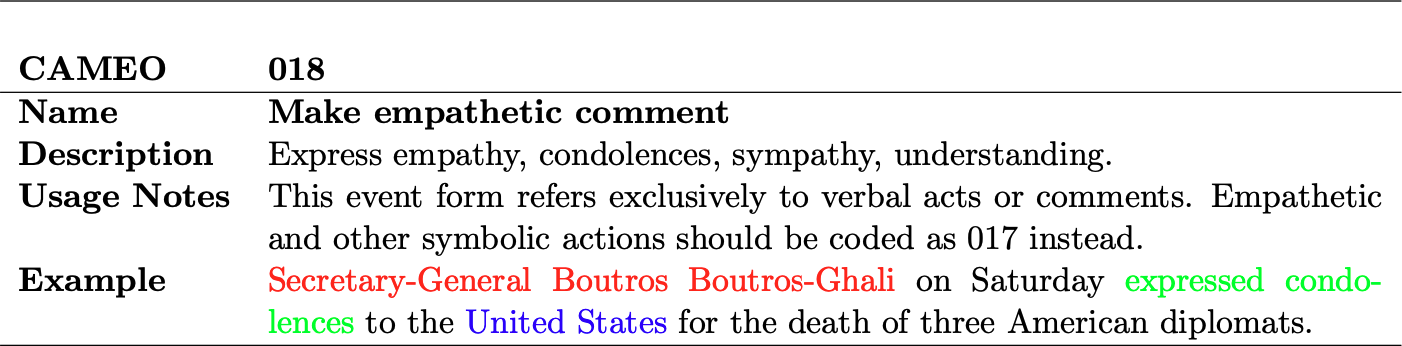
\includegraphics[width = \textwidth]{cameo.png}
   }
   \only<5>{
      \framesubtitle{Global Knowledge Graph}
      \begin{itemize}
         \item GKG is an array of highly sophisticated natural language
         processing algorithms (sic!) to each document to compute a range of
         codified metadata encoding key latent and contextual dimensions of the
         document.
         \item Among others these fields inform about:
         \begin{enumerate}
            \item Date;
            \item Source;
            \item Themes;
            \item Locations;
            \item Organizations;
            \item Persons;
            \item Tone.
         \end{enumerate}
      \end{itemize}
   }
\end{frame}

\section[Migration Studies]{Migration Studies}

\begin{frame}
   \frametitle{Societal response to Ukrainian refugee migration}
   \only<1>{
      \framesubtitle{Weisser, 2022}
      \begin{itemize}
         \item Eight weeks after the first shot was fired, the overall number of
         Ukrainians seeking protection abroad stood at \alert{5.1 million}
         (UNHCR, 2022).
         \item Whilst the \alert{influx of (large) refugee populations is typically
         associated with positive impulses for the local economy}, attitudes towards
         refugees and political preferences of native residents edge towards a more
         hostile position. 
         \item Attitudes towards refugees may also be shaped by news media
         consumption (De Coninck, 2020).
         \item Overall, societal attitudes towards refugees depend strongly on the economic and institutional setting.
         \item Concomitantly, changing attitudes have the potential to shape the
         politico-economic environment in host countries.
      \end{itemize}
   }
   \only<2>{
      \framesubtitle{Research question}
      \begin{block}{}
         How did the description of the Ukrainina refugee changed as the effect of
         the Russian invasion of Ukraine?
      \end{block}
   }
   \only<3>{
      \framesubtitle{Method}
      \begin{itemize}
         \item Data from the GDELT event database over \alert{16 weeks, starting with 30 December 2021}.
         \item Within the sample of European primary actors with unambiguous
         country affiliations, there are \alert{58,007 recorded events} with
         refugees as secondary actors.
         \item Each retrieved interaction event between a European primary actor
         and refugees is classified according to one of the following four
         modes:
         \begin{enumerate}
            \item Verbal cooperation;
            \item Material cooperation;
            \item Verbal conflict;
            \item Material conflict. 
         \end{enumerate} 
      \end{itemize}
   }
   \only<4>{
      \framesubtitle{Weisser, 2022}
      \begin{figure}
         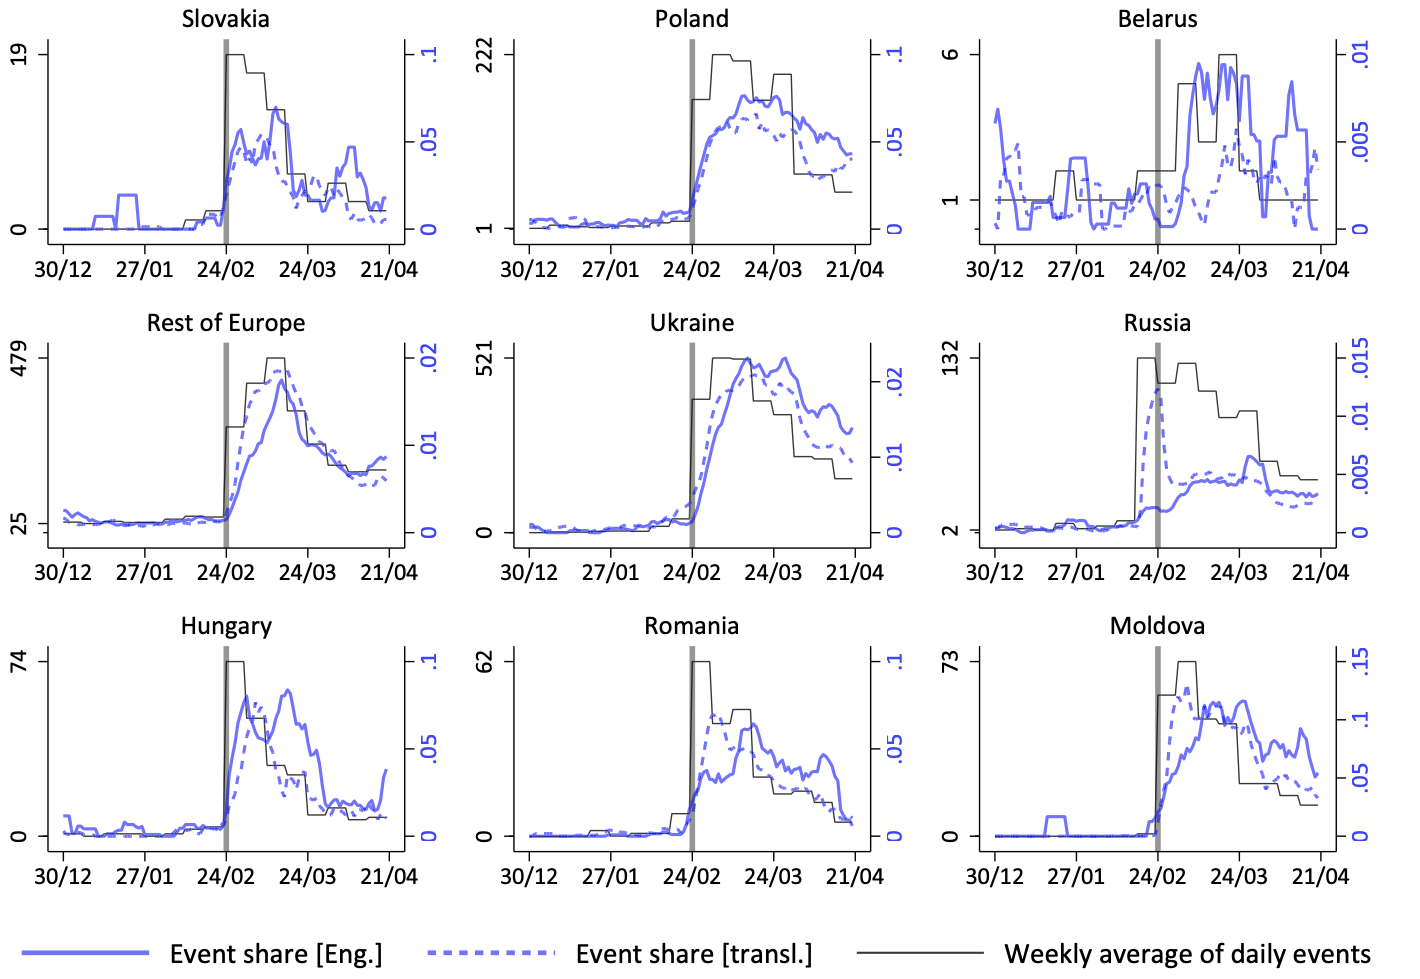
\includegraphics[width = \textwidth]{weisser_1.png}
      \end{figure}
   }
   \only<5>{
      \begin{figure}
         \framesubtitle{Weisser, 2022}
         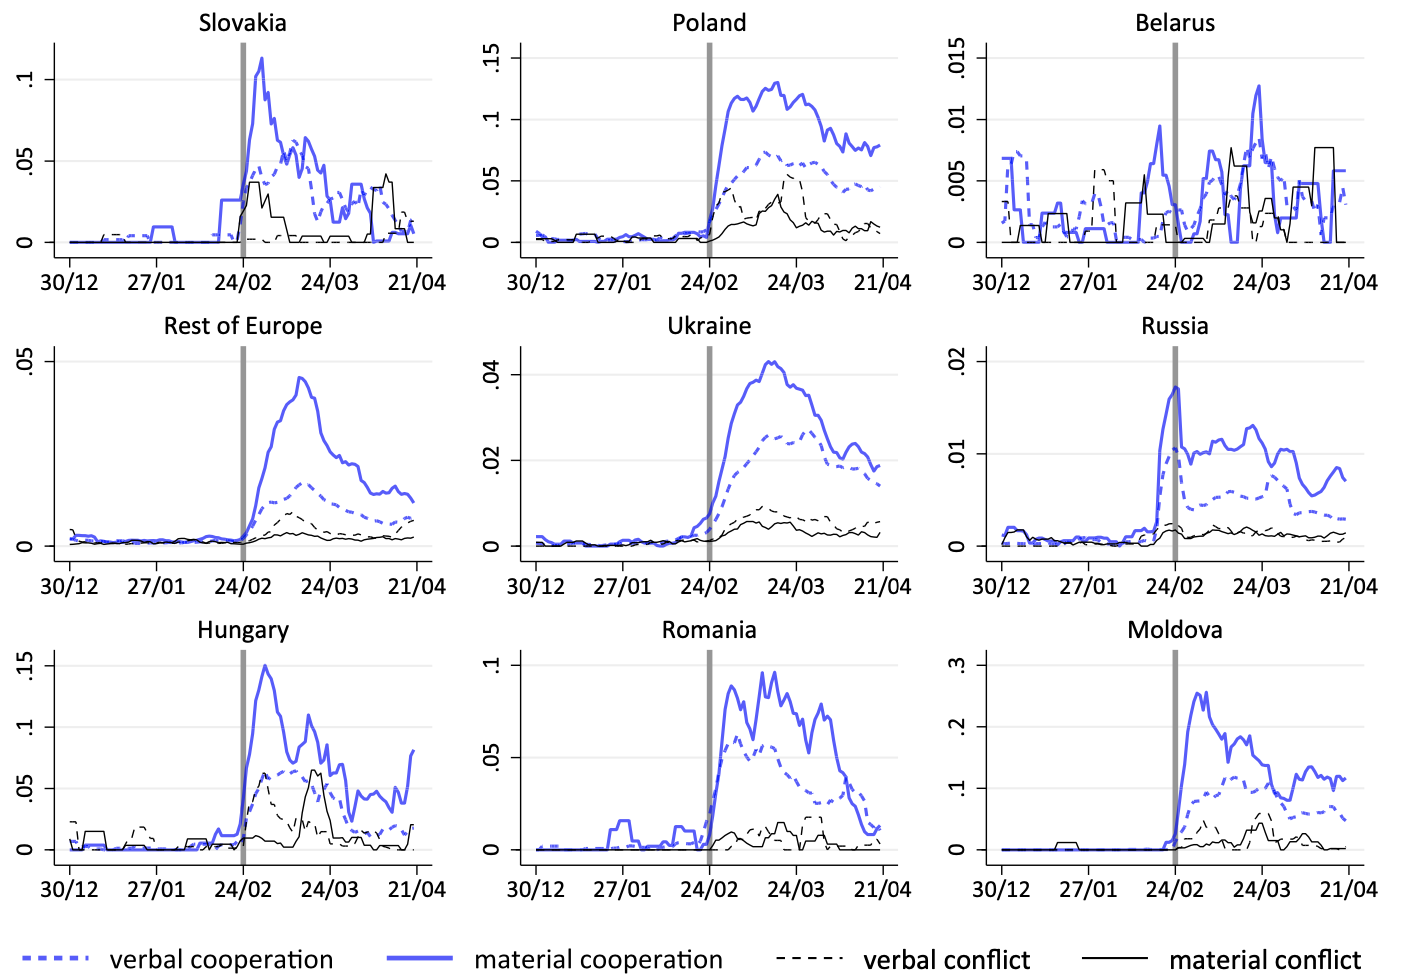
\includegraphics[width = \textwidth]{weisser_2.png}
         \caption{Weisser, 2022}
      \end{figure}
   }

\end{frame}

\section[GDELT API]{GDELT API}
\begin{frame}
   \frametitle{API}
   \only<+>{
      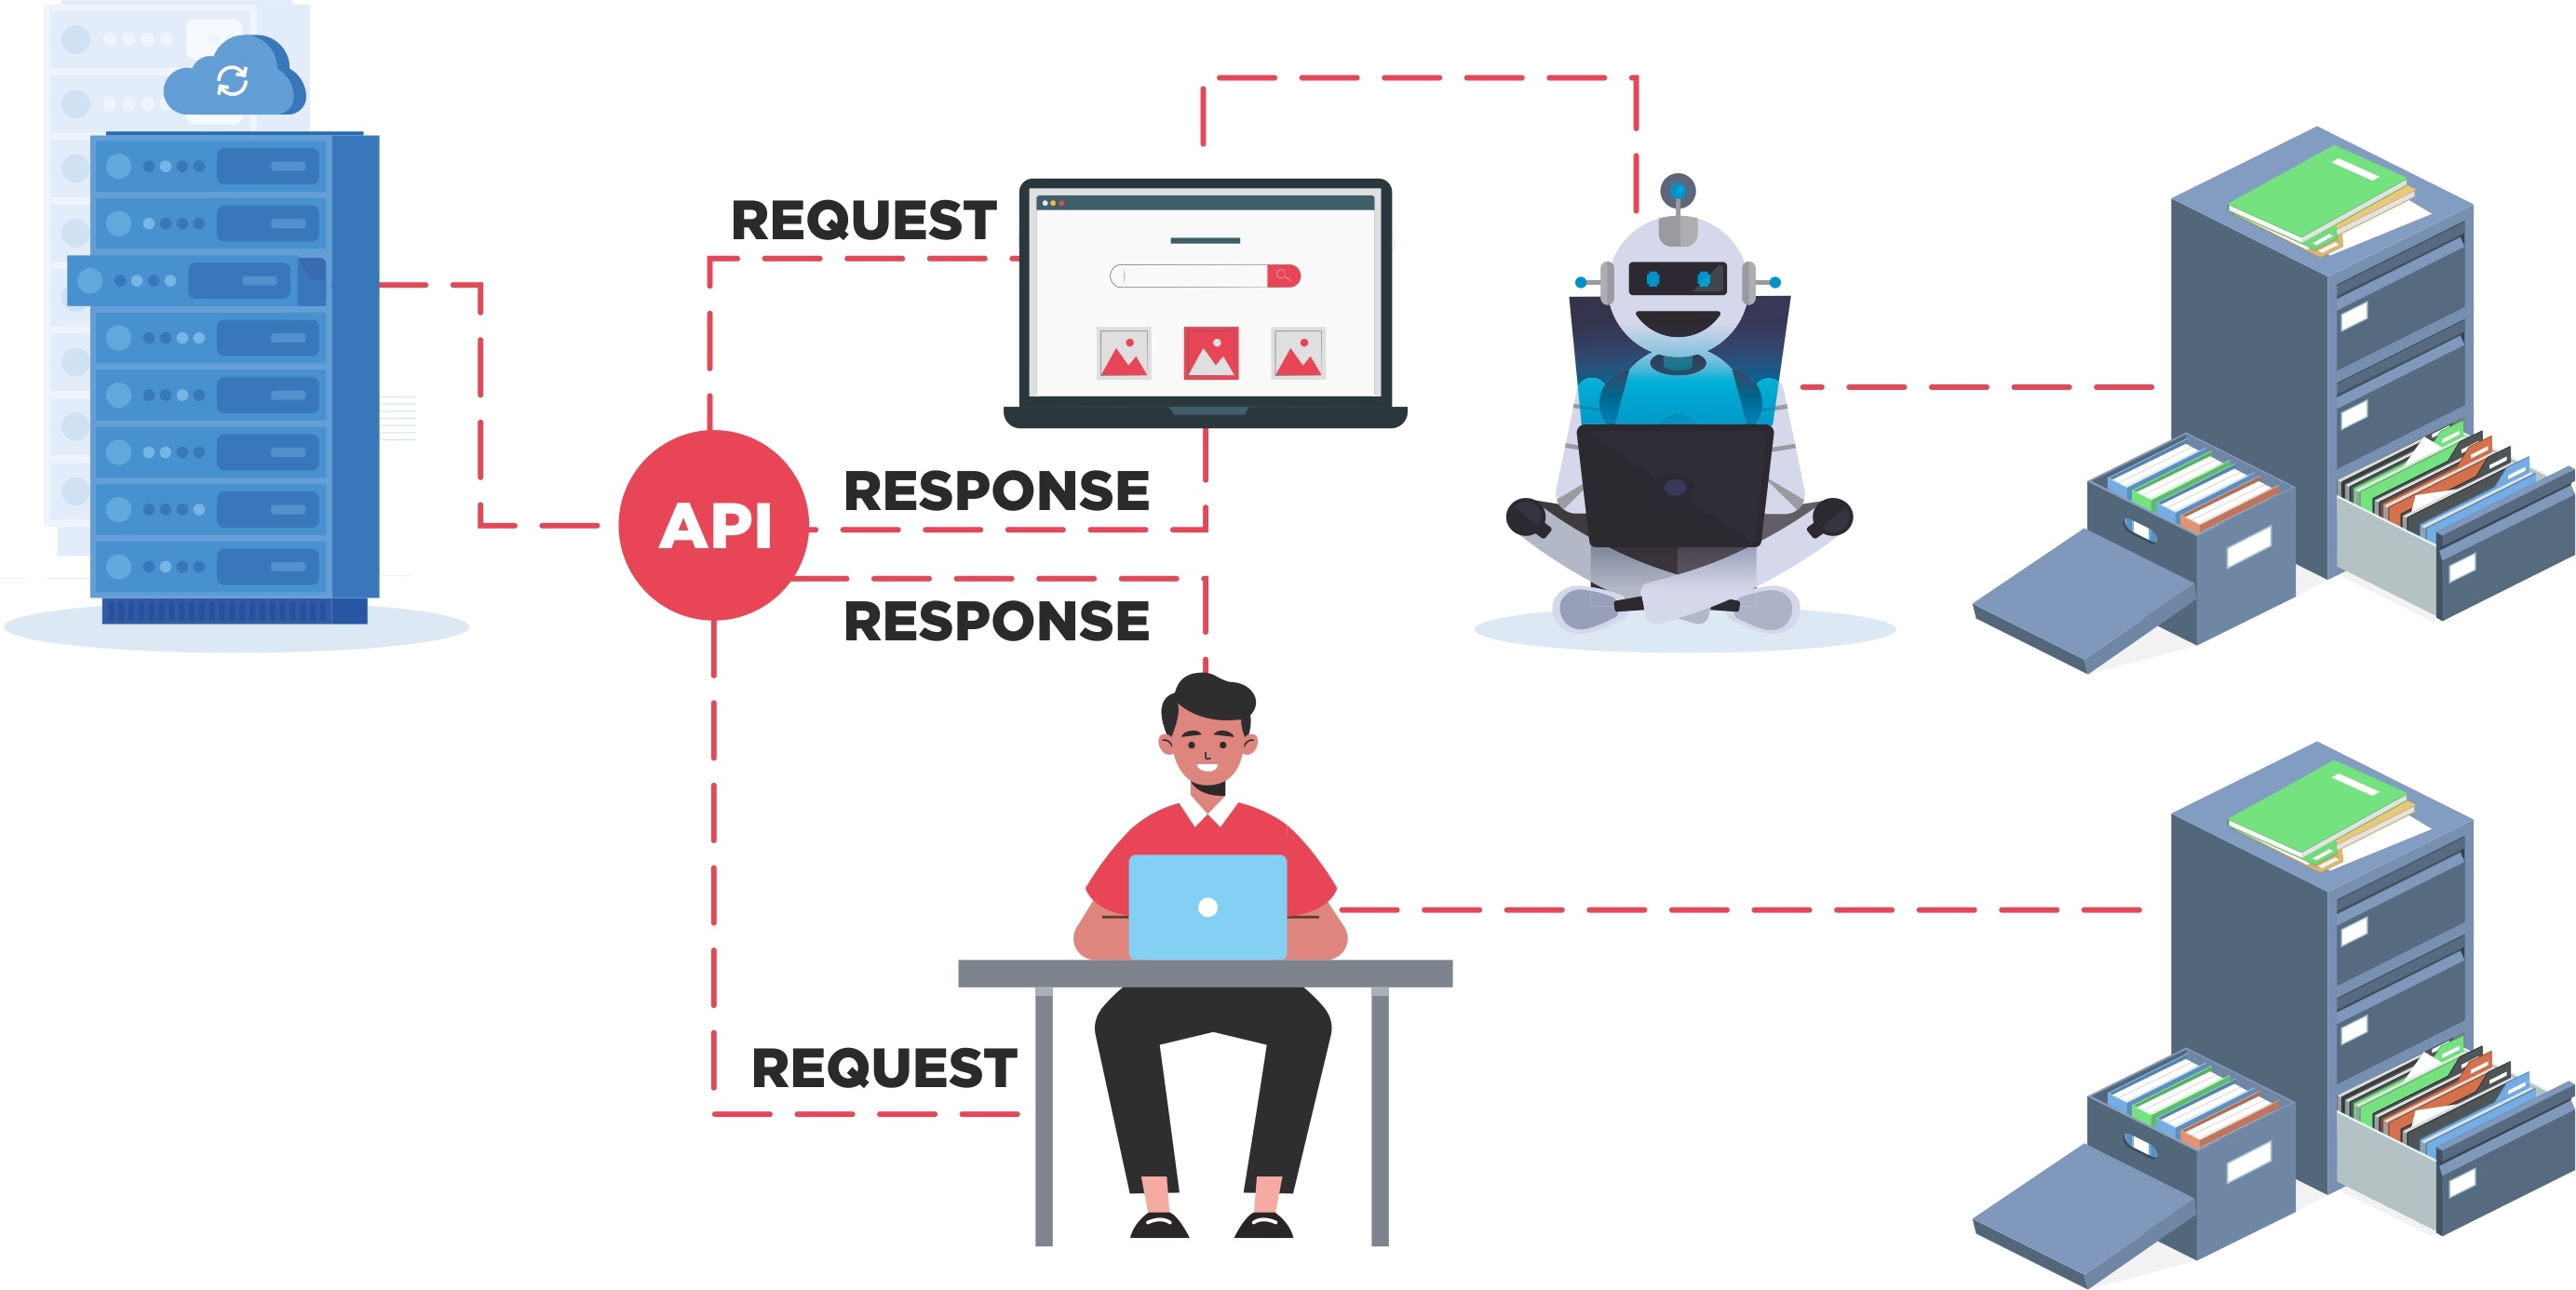
\includegraphics[width = \textwidth]{api.jpg}
   }
   \only<+>{
        \begin{definition}
            \emph{Aplication Programming Interface} is a communication protocol between a client and a server intended to simplify the building of client-side software. In other words, it is a contract between the client and the server which defines the format of possible requests and the format of the response (i.e. format of the data).
        \end{definition}
   }
   \only<+>{
      \framesubtitle{How to construct a request?}
      \begin{itemize}
         \item GDELT API Documentation is available at:
         \begin{center}
            \textcolor{blue}{\href{https://blog.gdeltproject.org/gdelt-doc-2-0-api-debuts/}{https://blog.gdeltproject.org/gdelt-doc-2-0-api-debuts/}}
         \end{center}
         \item The GDELT API lives under the following URL:
         \begin{center}
            \textcolor{blue}{\href{https://api.gdeltproject.org/api/v2/doc/doc?}{https://api.gdeltproject.org/api/v2/doc/doc?}}
         \end{center}
         \item The simplest request is constructed as follows:
         \begin{center}
            \textcolor{blue}{URL?}\textcolor{red}{query=ukraine}
         \end{center}
         \item You can add additional parameters to the request, such as:
         \begin{center}
            \textcolor{blue}{URL?query=ukraine}\textcolor{red}{\&mode=ArtGallery}
         \end{center}
      \end{itemize}
   }
   \only<+>{
      \framesubtitle{How to construct a request?}
      Construct a request using the GDELT API that will return:
      \begin{enumerate}
         \item Tone Chart about migrants;
         \item Tone Chart about refugees;
         \item Tone Chart about migrants in Polish media;
         \item Tone Chart about refugees in Polish media.
      \end{enumerate}
   }
   \only<+>{
      \framesubtitle{How to construct a request?}
      \begin{tikzpicture}
          \node at (0,0) {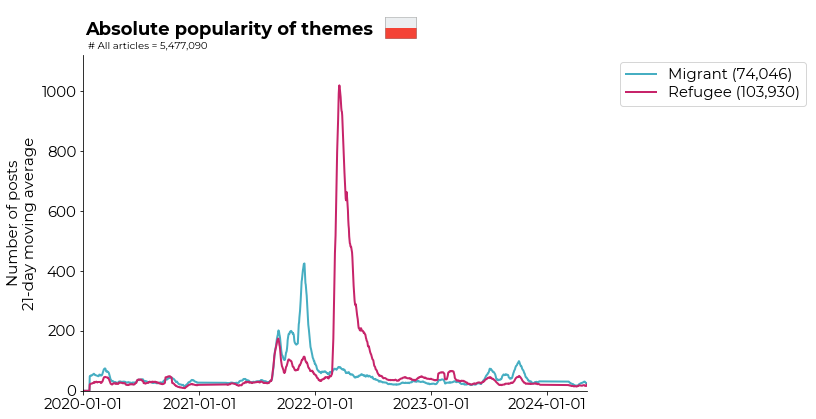
\includegraphics[width = 7cm]{pl_gdelt_themes_lines.png}};
          \node at (3.5,-3.75) {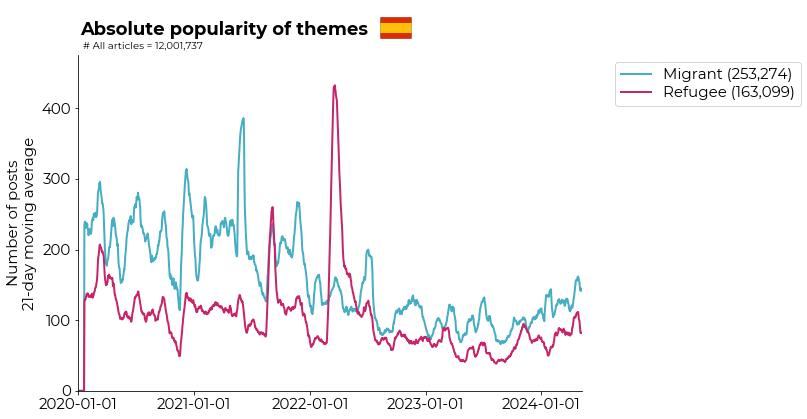
\includegraphics[width = 7cm]{esp_gdelt_themes_lines.png}};
      \end{tikzpicture}
   }
   \only<+>{
      \framesubtitle{How to construct a request?}
      Human-firendly interface for testing the API is avaliable at:
      \begin{center}
         \textcolor{blue}{\href{https://gdelt.github.io}{https://gdelt.github.io}}
      \end{center}
   }
\end{frame}


\end{document}